\chapter{Analysis \& Results}
\startcontents[chapters]
\printcontents[chapters]{}{1}{}
\noindent\\
So far the system's design, implementation, and example usage, has been presented and discussed.

\section{Introduction}
This chapter presents analytic information

\section{Implementation Analysis}
This section analysis the synthesised and implemented system-on-chip design to see the effect of increasing core counts.

\subsection{Design Size}
\subsubsection{Implementation}
On a minimal system-on-chip configuration, with one core and minimal peripherals and features (no reprogramming, no interrupts, no UART), the design requires as few as 700 LUTs with the processor core requiring approximately 300-400 LUTs.

\subsubsection{Memory Constraints}
As discussed in \cref{sec:singlecore} \nameref{sec:singlecore}, each processor core features two memories: instruction and scratch memory, which can both map onto synchronous, single-port, FPGA BRAM blocks. While this will reduce LUT requirements in designs with few cores, it becomes a non-trivial problem as the core counts increase. FPGAs have a fixed number of hard-BRAM blocks available for inference by the HDL compiler, for example the low-end Xilinx Spartan-6 XC6SLX9 FGPA features 32 18 Kb BRAM blocks \cite[p.~2]{s6fam}, and the Cyclone V 5CSEMA5F31C6N (used in the DE1-SoC) has 397 10 Kb blocks \cite[p.~22]{cvfam}.

\begin{figure}[h]
\begin{subfigure}{.5\textwidth}
  \centering
  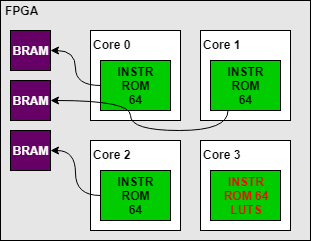
\includegraphics[width=.7\linewidth]{bram_limit}
  \caption{A theoretical FPGA device with 3 BRAM blocks running a 4-core design. Each core can map onto a BRAM block, however as there are more cores than BRAM blocks available, some core memories will be implemented as distributed RAM, or in the worse case using ALMs.}
  \label{fig:bram_limita}
\end{subfigure}%
\begin{subfigure}{.5\textwidth}
  \centering
  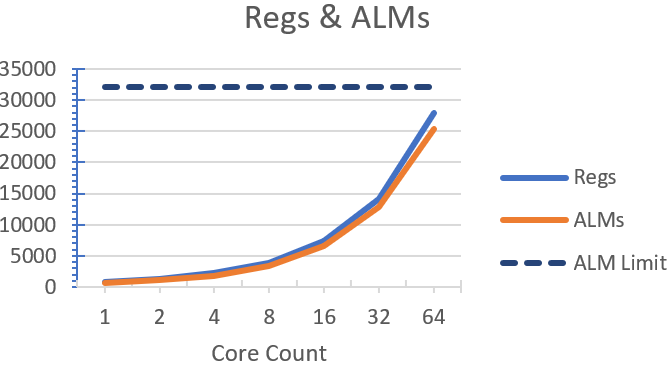
\includegraphics[width=1.2\linewidth]{sizes_regs}
  \caption{DE1-SoC (Cyclone V) resource utilisation with various core counts.}
  \label{fig:bram_limitb}
\end{subfigure}
\caption{}
\label{fig:bram_limit}
\end{figure}

As shown in \cref{fig:bram_limita}, as the number of processor cores increases, they eventually outnumber the available BRAM blocks resulting in their memories being implemented in either distributed RAMs or ALMs, both of which can consume significant logic resources of the FPGA which reduces the maximum possible core count.

Figure \cref{fig:bram_limitb} shows the FPGA resource requirements for the DE1-SoC board featuring the Cyclone V FPGA. Approximately 32 cores can be instantiated before the all the available registers and ALMs are consumed.

\subsubsection{Reducing Memory Requirements}
\label{sec:anal_memory}
As shown in \cref{fig:bram_limita}, each core has it's own instruction read-only memory. These memories have identical contents which presents an opportunity for optimisation. In the proposed design in \cref{fig:bram_limit_sola}, this memory is removed from each core and is instead available through a dedicated shared bus. This approach can be configured to be used in the Vmicro16 SoC through the \verb|DEF_CORE_HAS_INSTR_MEM| parameter in \verb|vmicro16_soc_config.v|, which enables the \textit{Instruction Memory Interconnect} shown in \cref{fig:watchdog}.

As shown in \cref{fig:bram_limit_solb}, the resource requirements using this shared memory approach is significantly less than having an instruction memory per-core. On the DE1-SoC, 64 cores can now be instantiated with a few thousand regs and ALMs left for other logic.


\begin{figure}[H]
\begin{subfigure}{.5\textwidth}
  \centering
  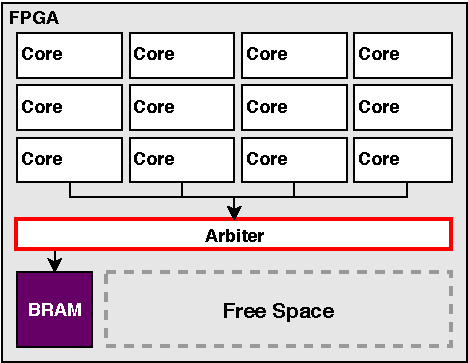
\includegraphics[width=.7\linewidth]{bram_limit_sol}
  \caption{A multi-core architecture where each core must fetch instructions externally from a global memory.}
  \label{fig:bram_limit_sola}
\end{subfigure}%
\begin{subfigure}{.5\textwidth}
  \centering
  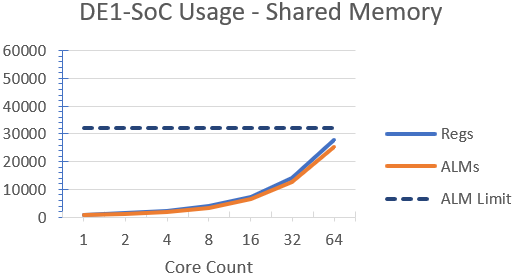
\includegraphics[width=1.2\linewidth]{sizes_regs_shared}
  \caption{DE1-SoC (Cyclone V) resource utilisation with various core counts using shared instruction memory.}
  \label{fig:bram_limit_solb}
\end{subfigure}
\caption{}
\label{fig:bram_limit_sol}
\end{figure}

Whilst this is a significant resource saving opportunity, it does have significant drawbacks. In the shared instruction memory approach, each core must now fetch it's instruction from the instruction memory interconnect which is subject to the arbiter and it's scheduling algorithm. The arbiter uses the same algorithm as the peripheral interconnect arbiter meaning that cores receive access incrementally, and as discussed in \cref{sec:multimaster}, this results in significant delays in many-core designs. This drawback is further explained in \cref{sec:result_results}.



\subsection{Maximum Frequency}
\cref{fig:sizes_fmax} below shows the maximum clock frequency for the design (Fmax) on the Cyclone V on the DE1-SoC. As expected, having more cores results in more logic and thus a longer  propagation delays to each core. System designers should consider the number of cores in their design as having fewer, faster, cores may outperform having more, slower, cores in some use-cases.

\begin{figure}[h]
\centering
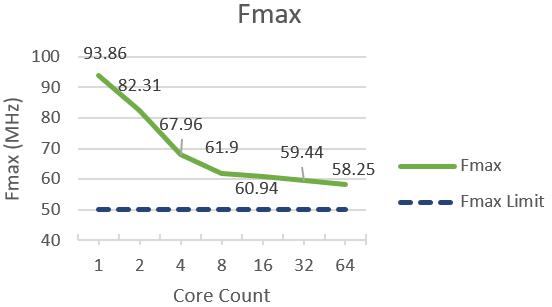
\includegraphics[width=0.6\textwidth]{sizes_fmax}
\caption{Cyclone V maximum design frequency for various core count configurations.}
\label{fig:sizes_fmax}
\end{figure}

\section{Scenario Performance}
To evaluate the performance of the system-on-chip, scenarios encompassing computational problems that are reflective of real-world applications are compiled and ran on the design.

\subsection{Scenario Overview}
\label{sec:scenario}
The scenario is a software program that runs a parallel implementation of the summation function, i.e. \verb|sum [1..10]| which returns 55. While this may seem too simple at first to measure performance of a multi-core system-on-chip, the function is actually quite appropriate as it encompasses various parallel problems, such as: a fixed time/size serial part; broadcasting of the data set (in this case the range of the summation); thread synchronisation (to know when the data is ready and to schedule gathering of intermediary results); and is highly scalable.
\\\\
The summation task flow is as follows:
\begin{enumerate}
\item Root (core \#0) broadcasts the range of the summation (i.e. sum 1 to 10) to all cores via the global shared memory.
\item Non-root cores wait for this broadcast to finish (memory barrier), then calculate their own subset of the range to sum. For example, if Root broadcasts that there are 240 samples and 10 cores in the system, each core calculates the subset size:

\begin{equation}
240/10 = 24
\end{equation} calculations starting from:
\begin{equation}
{ID_{CORE}} * 24
\end{equation}
For example, Core \#5 will start its 24 sample subset summation from
\begin{equation}
5 * 24 = 120
\end{equation}
effectively performing \verb|sum [120..123]|.

\item All cores perform an intermediary summation over their subset of the range (serial part).
\item All cores attempt to add their intermediary result to a global sum value in global shared memory (mutex).
\item All cores halt, signalling that their work has been committed to the global shared memory and have finished the program.
\end{enumerate}

This program is written in assembly in the file \verb|sw/demos/asm/sum64.s| and can be compiled using the assembly compiler (developed for deliverable \ref{ed:compiler}) using the command below. The assembly compiler outputs the file \verb|asm.s.hex| containing hex instruction words for use in Verilog's \verb|$readmemh| function. This data is used for each core's instruction memory. The assembly program is also shown in \cref{sec:64coresum}.
\\
\mintinline{bash}{                      python sw/asm.py sw/demos/asm/sum64.s}

\subsection{Performance Measurements}
Behavioural simulation is used to measure the following metrics to estimate general performance of the system-on-chip:
\begin{itemize}
\item Total program run-time.\\This is the time from when the reset signal is de-asserted to when all cores have halted. Each core has an output \verb|halt| signal which the SoC can use to determine if all cores have halted using \verb|wire all_halted = &core_halts;|. 

\item Time spent on the serial part.\\The serial part of this scenario consists of the intermediary summation of it's subset range. As each core is performing this task, the average will be used.

\item Time spent on communication.\\This includes time spent on thread synchronisation, i.e. waiting for the global memory to become available and waiting on the root to finish broadcast. Again, the average time will be used.

\item Time spent fetching instructions.\\Instruction fetches occur during stage \verb|STAGE_IF| of the pipeline. The behavioural test bench will record the number of clock cycles each core spends in this state, then calculate the average time spent fetching instructions. 
\end{itemize}

These measurements are recorded using non-synthesisable Verilog code in both the testbench and module code (\verb|vmicro16_soc.v|).

\subsection{Performance Results}
\label{sec:result_results}
The scenario program was simulated on system configuration with 1 to 30 cores with a 50 MHz clock.
\cref{fig:alg_time} shows the time breakdown of the multi-core system-on-chip running the scenario problem with various core counts. In these measurements all cores feature a small instruction memory which is accessed in constant time (one clock), and so this fetch time is not shown in the chart. 

\begin{figure}[h]
\centering
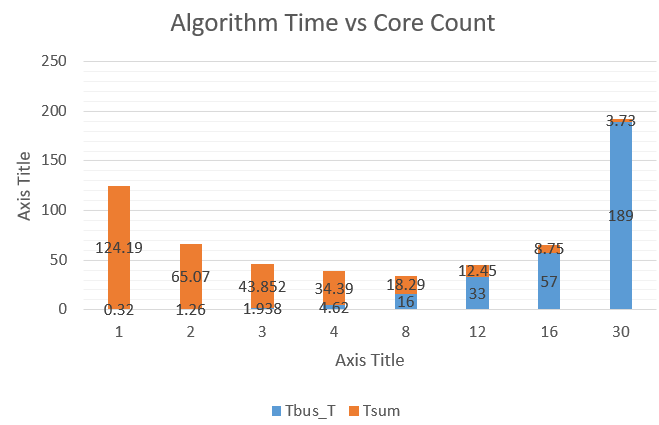
\includegraphics[width=0.7\textwidth]{alg_time}
\caption{Chart showing how the communication times (Tbus) and serial times (Tsum) changes with core count.}
\label{fig:alg_time}
\end{figure}

The chart shows the expected shape for software parallel performance -- as the number of cores increase, each core's problem space is reduced resulting in faster completion of the summation part, and an increasing amount of time is spent on thread communication. This result matches my CUDA and MPI parallelism performance analysis results conducted in 2018 \cite{soft354}.

It can be seen that the total run-time is fastest near 8 cores and increases at this point when using more cores. This is likely due to the small summation range per core -- with 30 cores just 8 samples per core are summed, which is extremely overkill and not representative of what a 30-core plus system should be used for.

If a much larger summation range was used (effectively representing a more appropriate scenario for systems with high core counts), the chart shape would stretch horizontally, resulting in the fastest time being on a higher core count than 8.

With high-core counts (16+) it can be seen that the communication time (Tbus\_T) increases significantly. This is likely due to the rotating arbiter design. As discussed in \cref{sec:multimaster}, the arbiter grants bus access to the next core incrementally after the previous core finishes. For large core systems, this can result in large time penalties. For example, if core \#30 is blocking all other cores and the arbiter is lagging behind granting access to core \#5, it will take a significant amount of time for the arbiter to reach core \#30 to unblock the system.

\subsection{Shared Instruction Memory Impact}
As previous discussed in \cref{sec:anal_memory}, using a shared instruction memory approach reduces the size of the design but will result in increasingly long instruction fetches as the core count increases. \cref{fig:alg_time_shared} below shows the same scenario but using shared instruction memory. The shape of the chart remains similar, however the total run-time is close to double the time of the per-core instruction memory results, and increases significantly with more cores.

\begin{figure}[h]
\centering
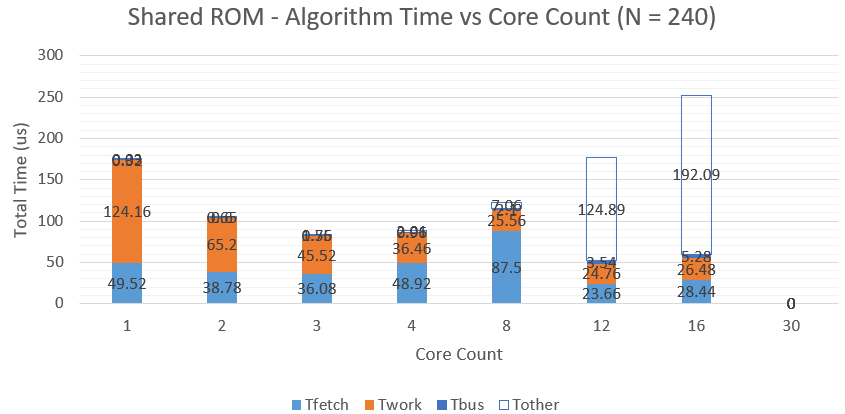
\includegraphics[width=0.7\textwidth]{alg_time_shared}
\caption{Similar to \cref{fig:alg_time} but using shared instruction memory to reduce block memory requirements per core.}
\label{fig:alg_time_shared}
\end{figure}

As with Figure \ref{fig:alg_time}, using too many cores for a small data set can result in the scenario taking longer than a single core.

\section{Analysis Review}
There are several takeaways from these results:
\begin{enumerate}
\item Use an appropriate number of cores for the dataset size.\\Too few cores result in longer work times and shorter communication times, and too many cores results in shorter work times and longer communication times.

\item Use an appropriate arbitration scheme to prevent blocking the system for too long.\\
In this design, and likely others, the blocking core is known by the global shared memory (via the locking cells) meaning that this information can be passed to the arbiter to give priority, while still avoiding deadlocks, to the blocking core.

\item Use an appropriate number of cores and still have space for other business logic.

\item More cores may result in lower clock frequencies.\\From \cref{fig:sizes_fmax}, the single-core design can be ran at $\approx$95 MHz while the 4-core design only $\approx$65 MHz (a $\approx$30\% decrease). The parallel speed improvements from having more cores may be less than a single fast core.
\end{enumerate}

System designers should experiment with their algorithm and these takeaways to determine the approximate number of processor cores for their requirements, be that algorithm time, size, clock frequency, or compilation time.



\chapter{Conclusion}
\startcontents[chapters]
\printcontents[chapters]{}{1}{}

\section{Review Against Project Deliverables}
\subsection{Core Deliverables}
This project has achieved all core deliverables outlined in \cref{sect:goals} \nameref{sect:goals}.

\begin{enumerate}[leftmargin=2\parindent, label=\bfseries CD\arabic*]
\item{\textbf{Design a compact 16-bit RISC instruction set architecture.}\\
\textit{Achieved}. A new 16-bit instruction set has been designed and implemented, nicknamed \textit{Vmicro16} (Verilog microprocessor 16-bits).
}

\item{\textbf{Design and implement a Verilog RISC core that implements the ISA in \ref{cd:isa}.}\\
\textit{Achieved}. The implementation is found in \verb|vmicro16.v|.
}

\item{\textbf{Design and implement an on-chip interconnect for multi-core processing (2 to 32 cores) using the RISC core from \ref{cd:core}.}\\
\textit{Achieved}. The AMBA APB bus was chosen and adapted for multi-master support. While the design is simple and lacks in performance, it does not consume a significant amount of area, leaving space for more cores and peripherals.
}

\item{\textbf{Analyse performance of serial and parallel software algorithms, such as parallel DFT, on the processor.}\\
\textit{Achieved}. A summation computation was chosen to demonstrate effectiveness in various parallel computational problems, such as subset calculation, thread communication, and broadcast/gather procedures.
}

\item{\textbf{Allow the RISC core to be easily compiled to multiple FPGA vendors (Xilinx, Altera).}\\
\textit{Achieved}. The design has been successfully compiled on Quartus Prime, Xilinx Vivado, Xilinx ISE, ModelSim, and Icarus Verilog. The design has been succesfully implemented on the Cyclone V and Spartan-6 FPGA devices.
}
\end{enumerate}

\subsection{Extended Deliverables}
\begin{enumerate}[leftmargin=2\parindent, label=\bfseries ED\arabic*]

    \item{\textbf{Design a RISC core with an instructions-per-clock (IPC) rating of at least 1.0 (a single-cycle CPU).}\\
    \textit{Not achieved}. Although present in the interim update, it was decided to remove this feature due to it's complexity and possibility of it hindering multi-core and interrupt integration.
    }
    
    \item{\textbf{Design a RISC core with a pipe-lined data path to increase the design's clock speed.}\\
    \textit{Achieved}. Data in the processor's pipeline is clocked through stages of flip-flops to reduce the critical path.
    }
    
    \item{\textbf{Design a scalable multi-core interconnect supporting arbitrary (more than 32) RISC core instances (manycore) using Network-on-Chip (NoC) architecture.}\\
    \textit{Not achieved}. The implemented design uses traditional multi-core communication techniques (shared memory communication, mutexes, etc.) rather than a NoC architecture. While the NoC design would be more scalable, it would be of much higher complexity and therefore out-of-scope for this project's timeline.}
    
    \item{\textbf{Design a compiler-backend for the PRCO304 \cite{prco304} compiler to support the ISA from \ref{cd:isa}. This will make it easier to build complex multi-core software for the processor.}\\
    \textit{Somewhat achieved.} While a compiler backend was produced that allowed high-level code to be compiled and run on the Vmicro16 processor, it lacked many multi-core and interrupt features. In addition, many unforeseen bugs were found in the original compiler, and it was decided instead to build and use a simpler text-assembly based compiler, \verb|asm.py|.
    }
    \item{\textbf{The RISC core can communicate to peripherals via a memory-mapped addresses using the Wishbone bus.}\\
    \textit{Achieved.} Although not Wishbone, AMBA APB was used instead as I it's interface is more intuitive.}
    
    \item{\textbf{Implement various memory-mapped peripherals such as UART, GPIO, LCD, to aid visual representation of the processor during the demonstration viva.}\\
    \textit{Somewhat achieved.} Modular UART, GPIO, watchdog, bus recovery, and memory peripherals were created to visually demonstrate features of the design. An LCD peripheral was not made due to time-constraints, however it would have been beneficial to do so to demonstrate conditional compilation for different development boards. A collection of software demos utilising these modules can be found in \cref{sec:vivademos}.}
    
    \item{\textbf{Store instruction memory in SPI flash.}\\
    \textit{Not achieved.}}
    
    \item{\textbf{Reprogram instruction memory at runtime from host computer.}\\
    \textit{Achieved.} The global instruction memory (if enabled, see \cref{sect:config}) supported run-time programming over the UART0 interface. An example host-programmer application is provided in \verb|sw/prog.py|.}
    
    \item{\textbf{Processor external debugger using host-processor link.}\\
    \textit{Not achieved}.}
\end{enumerate}


\section{Future Work}
There are several aspects to this project which could be improved. First, 













